\section{XSnare Design}

 \begin{figure*}[h]
	\begin{subfigure}[b]{1.0\textwidth}
		\centering
		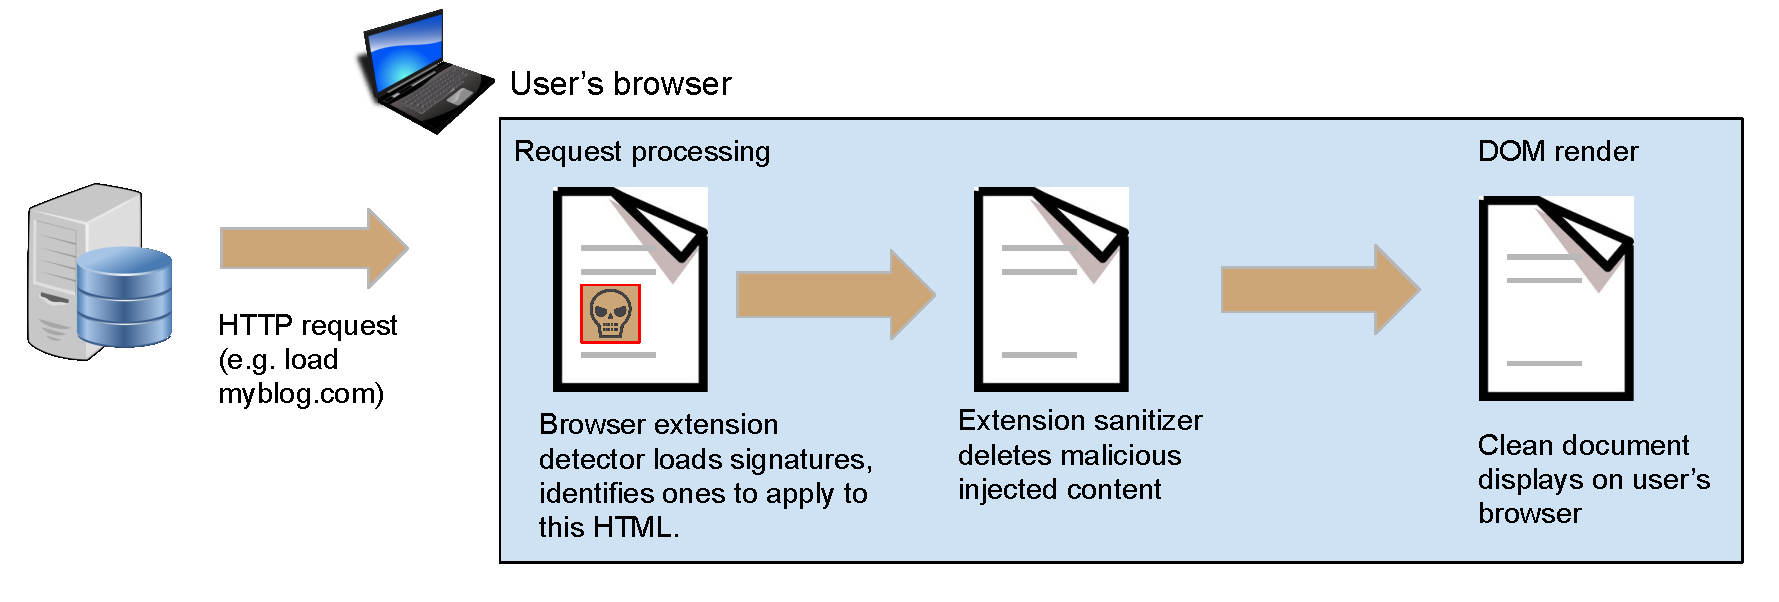
\includegraphics[scale=0.55]{img/xsnare_top.pdf}
		
	\end{subfigure}
	\hfill
	\begin{subfigure}[b]{0.3\textwidth}
		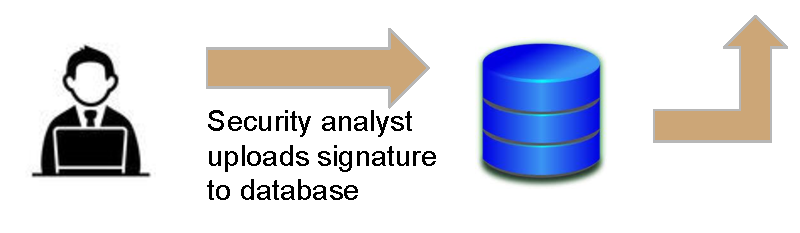
\includegraphics[scale=0.55]{img/xsnare_bot.pdf}
		
	\end{subfigure}
	\caption{XSnare's approach for protection against XSS.}
	\label{fig:xsnare}
\end{figure*}

We now present XSnare's components and how they interact with each other.

\subsection{Operation, at a glance}
  Figure~\ref{fig:xsnare} illustrates how the firewall can be used to guarantee full client-side protection: A user loads a request, such as \url{www.myblog.com}, this request might come back with malicious code in the form of an XSS attack. Before rendering the webpage in the browser, an extension can analyze the potentially malicious document. First, it loads signatures which a security analyst (a bug bounty hunter, for example) has uploaded to a database. The extension's detector analyzes the given HTML string and identifies the signatures which apply to this document. The signatures specify the injection spots in the document, and the extension's sanitizer gets rid of any malicious content. Finally, the extension returns a clean HTML document, which the browser then renders. TODO: Section x explains our algorithm in detail
 



\iffalse
 \begin{figure*}[h]
 	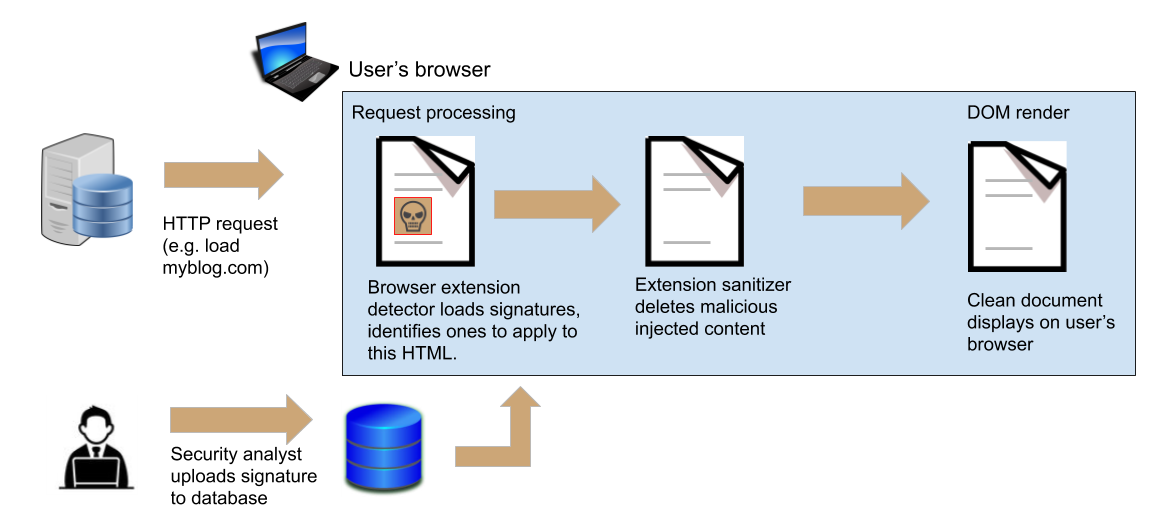
\includegraphics[scale=0.55]{img/xsnare.png}
 	\caption{XSnare's approach for protection against XSS.}
 	\label{fig:dom_firewall}
 \end{figure*}
\fi

\subsection{An example application of XSnare}

In order to further explain this approach, we present a small example of how DOM context can be used to defend against XSS, taken from CVE 2018-10309 \cite{examplecve}. This is reproducible in an off-the-box WordPress installation running the Responsive Cookie Consent plugin, v1.7. This is also an example exploit which Chrome's XSS auditor does not protect against. Consider a website running PHP on the backend that takes user input and stores it to later display it to another user; in this case, the input element's value attribute is set by the webpage admin using the plugin's UI.

The PHP code defines the static HTML template (in black) in the "admin-page.php" file, as well as the dynamic input (in red):

\begin{lstlisting}
<input id="rcc_settings[border-size]" 
name="rcc-settings[border-size]" 
type="text" value=<@\textcolor{red}{"<?php rcc\_value('border-size'); ?>"}@>/>
<label class="description"
for="rcc_settings[border-size]">
\end{lstlisting}
\
\\
This HTML will be displayed in the admin's UI. Under normal circumstances, the input element might be used to insert a value of "0" as the dynamic content:
\\
\begin{lstlisting}
<input id="rcc_settings[border-size]" 
 name="rcc-settings[border-size]" 
 type="text" value=<@\textcolor{red}{"0"}@>>
<label class="description"
 for="rcc_settings[border-size]">
\end{lstlisting}
However, the php code is vulnerable to an injection attack, as it is not sanitized on the server side. If we have
\begin{lstlisting}
border-size = ""><script>alert('XSS')</script>
\end{lstlisting}
then, the browser will render the following, executing the injected script:
\begin{lstlisting}
<input id="rcc_settings[border-size]" 
name="rcc-settings[border-size]" 
type="text" value=<@\textcolor{red}{""><script>alert('XSS')</script>}@>
<label class="description"
for="rcc_settings[border-size]">
\end{lstlisting}

Note that this HTML is well-formed, so it is hard to detect that a malicious injection has occurred without knowing the developer's intention. However, assuming an analyst has knowledge of how the full HTML should render without any injections, and the possible range of values of the injection, they can single out the point of injection, by separating user input from the server-side template, and get rid of the malicious script entirely. In the example, the injected script in red can be easily distinguished from the rest of the HTML template due to their identifiable attributes. By searching for this specific input element from the top of the document, and this label element from the bottom, the dynamic content can be identified from the static template.

When sanitizing the injection points, we would ideally sanitization functions that are equivalent to the server-side patch, but the application developer's intention might not always be clear. After careful analysis of the code in the example, we noted that while the CVE describing this vulnerability states that the bug was fixed in version 1.8 of this plugin, this was not the case: the developer fixed other similar vulnerabilities but did not handle this specific parameter. However, we can infer the application's intended behaviour from the other patches \cite{rccpatch}. In particular, the developer applied a built-in WordPress function "sanitize\_text\_field", which sanitizes the parameters by checking for common invalid characters like invalid UTF-8. The task of determining the intended behaviour falls upon a security analyst, who will act as the signature developer for a given exploit.  

In the following sections we give a detailed description of each component of our system, the challenges that arise when trying to defend against XSS client-side, and the tools provided by the browser to facilitate our methods. 
 
 \subsection{Firewall Signatures}
	 The firewall signatures are at the core of our defense strategy. These must be precise enough for our system to get rid of the intended injection, and not an element of the website crucial to the user experience. Since we are only relying on DOM knowledge, these signatures must be related to HTML features, for example, specifying elements and element attributes that are unique to where the exploit might occur. 
	 
	 The basis for our signatures relies on two observations: first, an injection has a start and end point, that is, an element can only be injected between a specific HTML node and its immediate sibling in the DOM tree; second, in a well-formed DOM, the dynamic content will not be able to rearrange its location in the document without any JavaScript execution (e.g. removing and adding elements), allowing us to isolate it from the template code. Thus, our basic approach at signature definition is to specify an injection's start and its end, and any sanitization to be done between these two endpoints. Typically, one page will have several dynamic content injection points. The signature developer has to be able to identify all of these. Different scenarios might warrant different resolutions, ranging from stopping a webpage's rendering altogether, to performing some basic checks on the string. We discuss how different exploits might affect a signature definition and how our signature language gives an analyst enough expressibility to deal with these in later sections.
	 
	 We believe CVEs to be an ideal source for signatures, and our system assumes these are written by a third-party: as discussed previously, bug bounty hunters and penetration testers will commonly identify issues in application code, inform developers and publish it for the benefit of the community in the form of CVEs. Our system adds an extra component to this workflow, where hackers and security enthusiasts also write the signatures to defend users. Thus, the signature database is maintained by a trusted entity which audits CVEs, and thus, a malicious analyst can not take advantage of this model to throttle the extension's performance. An analyst can write a signature in our language given their knowledge on the exploit, as they will often know both the source and the way it manifests in the HTML, as well as the fix.
 
 \subsection{Firewall Signature Language}
 Our signature language needs to be such that it has enough power of expression for the signature writer to be precise, both for determining the correct web application and to identify the affected areas in the HTML. Due to the nature of our signature definitions, a regex language suffices to express precise sections of the HTML. Furthermore, a regex language allows us to identify malformed HTML before it renders on the browser. The following is the signature that defends against the motivating example of Section 2.1:
 \lstset{basicstyle=\small}
\begin{lstlisting}
url: 'wp-admin/options-general.php?page=rcc-settings',
software: 'WordPress',
softwareDetails: 'responsive-cookie-consent',
version: '1.5',
type: 'string',
typeDet: 'single',
sanitizer: 'regex',
config: '/^[0-9](\.[0-9]+)?$/',
endPoints: 
['<input id="rcc_settings[border-size]" 
name="rcc_settings[border-size]" type="text" value="',
'<label class="description" 
for="rcc_settings[border-size]">']
\end{lstlisting}
 
 Along with the previously mentioned endpoints, the signature also defines the urls, if necessary, in which the exploit occurs, what kind of webpage it is (WordPress in this case), and any additional details of the software. In this case, since it's a WordPress site, the details include the description of the vulnerable plugin. The \texttt{typeDet} value specifies whether this signature includes a "single" pair of endPoints, or "multiple". This is useful for when one signature developer has identified several vulnerable points in the same document, and the writing can be streamlined into one signature. Having multiple injection points in one document complicates the detection mechanism: for example, if one document has two different injection points, a knowledgeable attacker might leverage this information to try to trick the extension into identifying the wrong spots. We further discuss measures to protect against these attacks in the implementation section.
 
 Once the dynamic content is identified, the analyst can configure their signatures with a function chosen from a pre-defined static set of sanitization functions. These functions innoculate potential malicious injections based on the DOM context surrounding the injection. The goal of signatures is to provide such sanitization, while maintaining the core web page user experience. To this end, default injection point sanitization is done with DOMPurify \cite{10.1007/978-3-319-66399-9_7}. This library is described by its creators as a "DOM-only, super-fast, uber-tolerant XSS sanitizer for HTML, MathML and SVG". The Mozilla community cites it as an useful tool for "safely inserting external content into a page" \cite{safecontent}. While it offers a lot of configurability and hooks, we have used the default functionality, with satisfying results, as described in Section 4, in our own signatures. However, there are cases where page functionality is lost due to a naive sanitization approach. Thus, it is sometimes more desirable to use a different sanitization approach, especially when heavier methods disrupt the look and feel of the web page.
 
  We provide different types of sanitization: "DOMPurify", "escape", and "regex". Regex Pattern matching can be particularly effective when the expected value has a simple representation, e.g. a name field should only have a particular subset of characters available. Additionally, for each of these approaches, the signature can specify a corresponding config value, as described in Section 5.1. DOMPurify provides a rich API for additional configuration. When escaping, defining specific characters to escape via regex can be useful. For pattern matching via regex, the config value specifies the string the injection point content should match.
 
 An alternative to this approach would have been to allow signatures to specify arbitrary code for the sanitization routines. While this would provide a more accurate sanitization technique, we have decided to impose a declarative spec for these routines for three main reasons:
\begin{enumerate} 
	\item Security Concerns: We assume signatures come from a trusted source. However, partly due to the way they are currently stored, it is possible for an attacker to add malicious signatures. In general, this would only cause pages to trigger signatures that should not have been triggered, potentially harming the web site user experience. If we allowed arbitrary code to run from signatures, an attacker could take control of the victim's browser, as the code would execute in a high-privilege environment.
	\item Case Coverage: While our provided methods might be limited in some scenarios, we have applied them in our studied CVEs with positive results, and are confident they can cover most use cases.
	\item Adoption: A declarative language will help signature developers expedite the process of writing signatures, as they will find that our provided methods will most often suffice.
\end{enumerate}
 
 \subsection{Firefox Extension}
 Our system's main component is a browser extension which rewrites potentially infected HTML into a clean document.
 We have decided to implement this tool as an extension due to the following main benefits:
 \begin{itemize}
 	\item \textbf{Ease of deployment and adoption}. Most modern browsers provide a convenient way to upload extensions to their respective official sites (Firefox Add-Ons in the case of Firefox). This eases deployment for the extension developer, and also eases installation for an user, as they can install the tool within the browser in one click, without having to install additional third-party software.
 	\item \textbf{Privileged execution environment}. The extension's logic can lie in a separate environment from the web application code. This is important for security, as it guarantees that any malicious code in the application can not affect the extension's behaviour. If the extension needs to run code within the application, it can maintain security by installing the code before the application's code runs. A web application, on the other hand, can not achieve this level of security in general, as it can not guarantee that its own code will run before any malicious code.
 	\item \textbf{Web application context}. Our solution requires knowledge of the application's context to perform several of its tasks. For example, it's useful to know which tab generated a network request to determine whether the response content is safe or not. The extension naturally retains this context.
 	\item \textbf{Ability to interpose at the network level and the web application level}. As it lies within the browser, the extension can run both at the network level, e.g. rewrite an incoming response or outgoing request; and at the web application level, e.g. keeping track of click events, or interpose on the application's JavaScript execution. Other types of solutions often have to choose between one or the other.
 \end{itemize}

Our extension's main purpose is to detect exploits in the HTML by using signature definitions and maintain a local database of signatures that is periodically updated from the main server.
The extension model provided by several browsers allows us to interpose on any functionality of a website in a privileged execution environment, unavailable to any third-party. In particular, Firefox provides the filterResponseData method through the webRequest API \cite{webRequest} . This allows the extension's background page to analyse and modify incoming network traffic. The extension translates signature definitions into the logic needed to rewrite incoming HTML on a per-URL basis, according to the top-down, bottom-up scan described earlier. 

The patch applied by the extension needs to take place in the raw HTML string. Even before any code runs, the parsing of the HTML into a DOM tree might cause elements to be re-arranged into an unexpected order, making our extension sanitize the wrong spot. For example, a <tr> element may only have direct children <th> or <td>. In our experiments, we found that an injection occurring as a direct child of the <tr> might cause the injected element to be rendered before the <tr> in the DOM. The following code shows the HTML as written in its file, with the injection (the img element) in red:

\begin{lstlisting}
<table class="wp-list-table">
  <thead>
     <tr>
     <th></th>
     <@\textcolor{red}{<img src="1" onerror="alert(1)">}@>
     <th>
   	    <form method="GET" action="">
...
\end{lstlisting}

According to this HTML, the signature developer might identify the exploit as occurring inside the table with the specified class, and the extension would be able to sanitize the code correctly. However, if we wait until the string has been parsed into a DOM tree, the elements are rearranged due to the previously mentioned rule:

\begin{lstlisting}
<@\textcolor{red}{<img src="1" onerror="alert(1)">}@>
<table class="wp-list-table">
   <thead>
   <tr>
   <th></th>
   <th>
      <form method="GET" action="">
...
\end{lstlisting}

Note that the injected img element is now outside of the table, simply by virtue of the DOM parsing. When performing the top-down search, the extension will search past the injection, as it occurs before the table element, and will therefore miss it during sanitization, creating a false negative. Similarly, false positives might occur if elements which were outside of an injection point are rearranged inside one. Thus, we can't wait until the website is rendered client-side to start interposing on code execution.

A knowledgeable attacker can therefore not take advantage of such behaviour: even if they know what the signatures look like, the extension can't be tricked into looking for the element in the wrong spot, as the injection can only happen after a signature's start and before its end. Additionally, the injection must end at a certain point in the document. Since we look for the end point from the bottom-up, we will eventually reach the injection's end, and, regardless of the contents (for example, trying to spoof the end point early), the sanitization will be correctly applied.


\iffalse
While we haven't seen any examples that warrant this functionality, it is possible for an exploit to only manifest itself through client-side dynamic behaviour, i.e. after an user clicks on the page. The network filter might not be able to defend against this, but the extension's content script can safely interpose on it through the user of event listeners and in particular Firefox's \textbf{beforescriptexecute} event, which occurs before a script element executes. Signatures can also be defined for these scenarios, to be ran in the content script. However, we believe this to be less ideal due to the added performance costs, as the extension now has to install the content script's code on all browser tabs.
\fi



